\chapter{Konzeption}

% Vorgehensweise oben anpassen

Um den \textit{SSD} und den \textit{YOLO} Objektdetektor miteinander vergleichbar zu machen und um deren Potential zum industriellen Einsatz zu bewerten, müssen konkrete Bewertungskriterien eingeführt werden. Mit Hilfe dieser Metriken werden die beiden Objektdetektoren anhand eines Benchmark Datensatzes initial verglichen, bevor der eigentliche Datensatz eingeführt wird. Dieser spiegelt Verhältnisse der Echtzeitumgebung wider. 

\section{Bewertungskriterien}

\subsection*{Präzision}

Um die Genauigkeit von Objektdetektoren zu messen, wird oft die Metrik \textit{mean Average Precision} (mAP) gewählt. Diese setzt sich aus zwei grundlegenden Größen zusammen (siehe Abbildung \ref{metrics}). 

\begin{figure}[ht]
	\begin{center}
		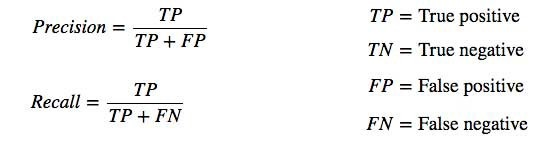
\includegraphics[width=10cm]{Bilder/metrics.png} 
		\caption[Precision und Recall Metrik]{Precision und Recall \cite{JonathanHui.20180307}}
		\label{metrics}
	\end{center}
\end{figure}

\textit{Precision} sagt also etwas über die Verlässlichkeit einer Klassifikation aus während \textit{Recall} Aussagen über die Erkennungsfähigkeit eines Objektdetektors trifft. Wichtig ist es hierbei anzumerken, dass mehrfach detektierte Objekte nur einmal als positiver Befund aufgefasst werden, die restlichen Detektionen gehen als \textit{False Positives} \cite{TarangShah.20180127}.

Die Klassifikation, ob eine Region das gewünschte Objekt enthält und demnach ein positiver Fall vorliegt, wird anhand des definierten \textit{IoU} Schwellwertes bestimmt. Dieser wird auch als \textit{confidence score} bezeichnet. Für den kompletten Datensatz werden nun für unterschiedliche \textit{confidence scores} jeweils \textit{Precision} und \textit{Recall} bestimmt und anschließend in einem Graphen aufgetragen. Meistens werden die \textit{confidence scores} so gewählt, sodass sich eine äquidistante Abstufung in den \textit{Recall} Werten ergibt \cite{TarangShah.20180127}. 

\begin{figure}[ht]
	\subfigure{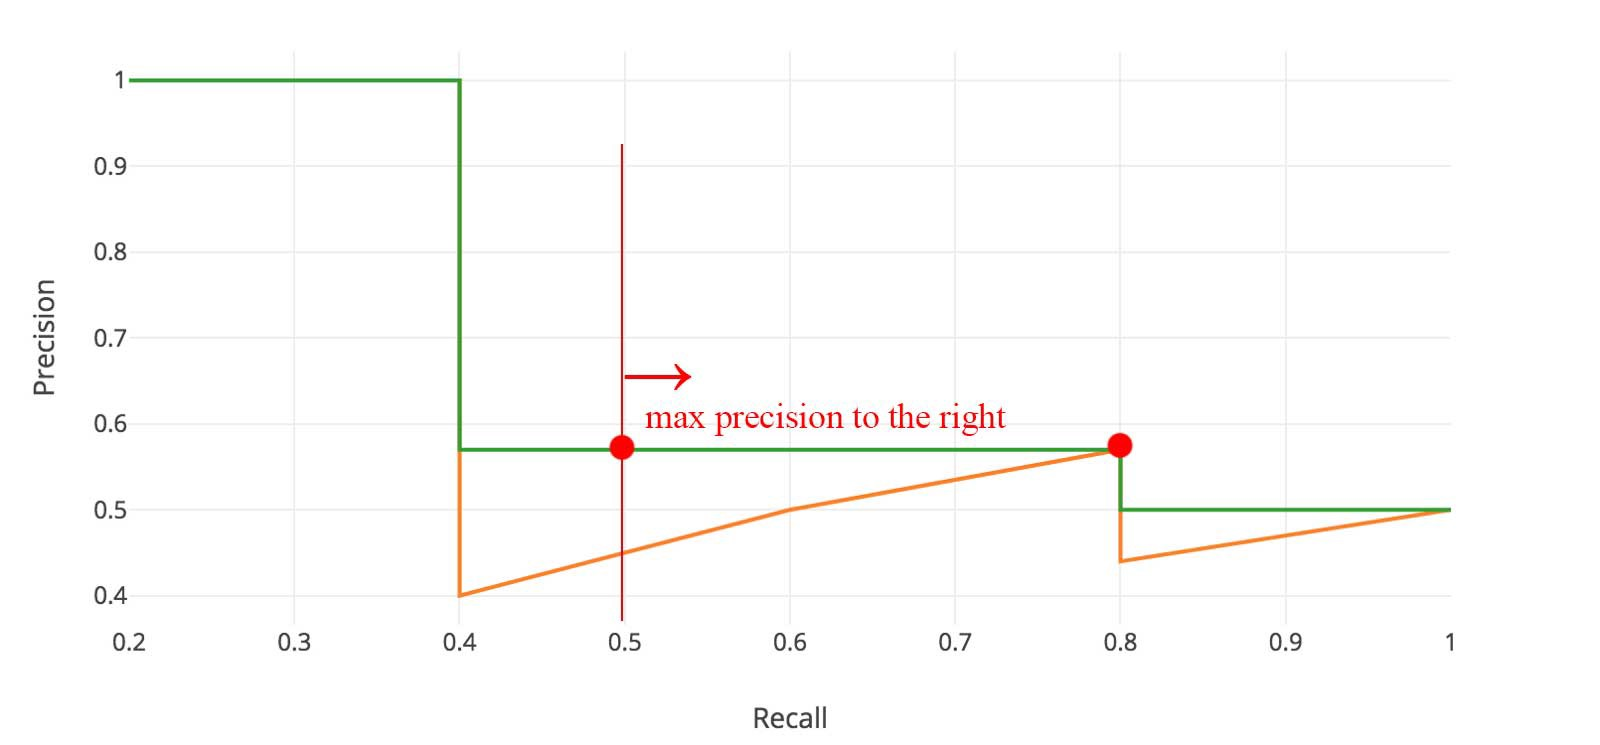
\includegraphics[width=7.5cm]{Bilder/map_graph1.png}} 
	\subfigure{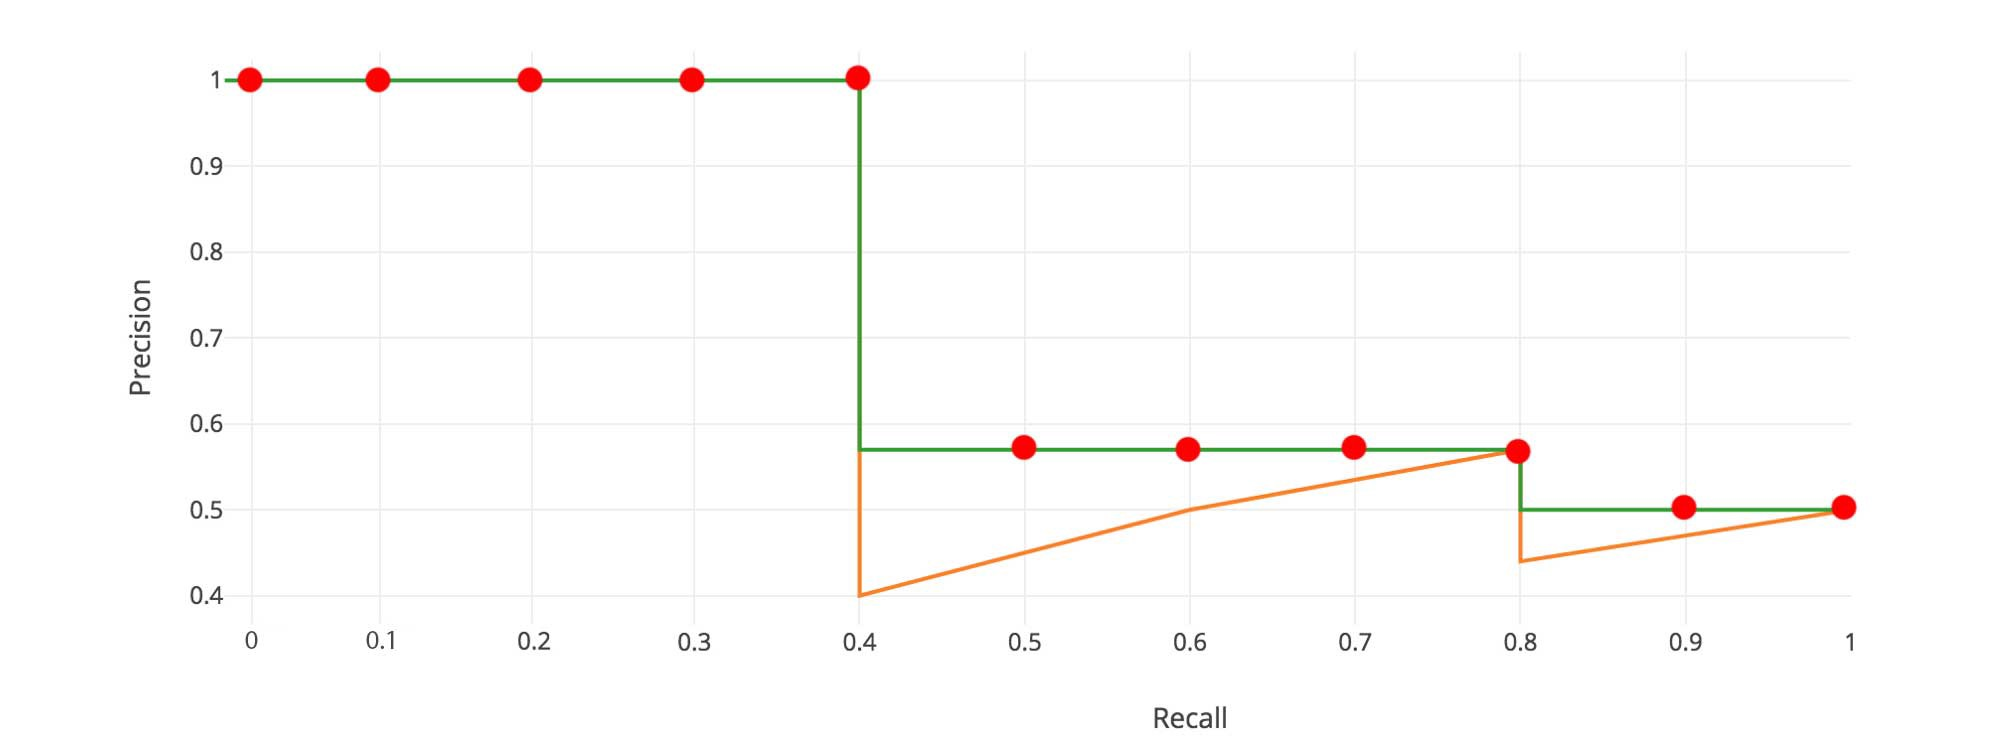
\includegraphics[width=7.5cm]{Bilder/map_graph2.png}} 
	\caption[Berechnung mAP]{Berechnung mAP \cite{JonathanHui.20180307}} 
	\label{map}
\end{figure} 

Im Graphen ist meist ein klassisches \glqq Zick-Zack\grqq{} Muster zu erkennen (siehe Abbildung \ref{map}). Dieses Muster wird geglättet, indem nach jedem Einbruch für jeden \textit{Recall} Wert der maximale \textit{Precision} Wert rechts des aktuellen \textit{Recalls} übernommen wird. Wird anschließend das diskrete Integral über alle \textit{Recall} Werte gebildet, so ergibt sich der \textit{Average Precision} Wert für eine zu klassifizierende Kategorie. Der Mittelwert der  \textit{Average Precisions} über alle Klassifikationskategorien hinweg ergibt letztendlich den \textit{mAP} Wert \cite{JonathanHui.20180307}. 

\subsection*{Reaktionsvermögen}

Um eine Verarbeitung in Echtzeit zu ermöglichen muss gewährleistet sein, dass die Interferenz mit dem Modell mit der eingehenden Bildrate einhergeht. Als Maßstab dafür dient die \textit{Frames Per Second} (FPS) Zahl. Echtzeitfähigkeit im Projekt ist so definiert, dass die Bildrate der erzeugten Bilder mit den eingezeichneten Bounding Boxen nach der Interferenz mindestens so hoch sein muss wie die des eingehenden Bildstroms. 

\subsection*{Trainingsverhalten}

Unter dem Punkt Trainingsverhalten wird zusammengefasst, wie schnell sich die einzelnen Modelle mit den unterschiedlichen Objektdetektoren trainieren lassen. Hierbei wird besonderer Fokus darauf gelegt, wie viele Trainingsepochen notwendig sind, bis die Fehlerfunktion des neuronalen Netzes konvergiert. Es soll aber auch betrachtet werden, wie mit doppelt erkannten Objekten während des Trainingsprozesses umgegangen wird. 

\subsection*{Interaktionsverhalten}

Im Zuge der Evaluation des Interaktionsverhalten werden drei Kriterien betrachtet. Darunter fällt, wie die Objektdetektoren bei besonderen Beleuchtungsverhältnissen abschneiden. Dies beinhaltet sowohl unterbeleuchtete als auch überbeleuchtete Gegenden. Daneben sollen ebenso extreme Blicklagen ein Faktor sein, um zu evaluieren, wie gut sich die trainierten Objektdetektoren für den industriellen Einsatz eignen. Dies umfasst sowohl unter welcher Entfernung die Objekte betrachtet werden, als auch unter welchen Winkel. Zuletzt muss bewertet werden, wie gut Objekte erkannt werden können, die nicht vollständig zu erkennen sind. Dies ist der Fall, wenn Objekte hintereinander angeordnet sind oder durch andere Beilagen verdeckt sind. 
